\documentclass[border=10pt]{standalone}
\usepackage{tikz}
\usetikzlibrary{arrows.meta}
\tikzset{%
  >={Latex[width=2mm,length=2mm]},
  % Specifications for style of nodes:
            base/.style = {rectangle, rounded corners, draw=black,
                           minimum width=3cm, minimum height=1cm,
                           text centered, font=\sffamily},
       bluebox/.style = {base, fill=blue!15}, %blue!30
       redbox/.style = {base, fill=red!30}, %red
       greenbox/.style = {base, fill=green!30}, %green
       process/.style = {base, minimum width=2.5cm, fill=orange!30, %orange!15
                           font=\ttfamily},
}

\begin{document}
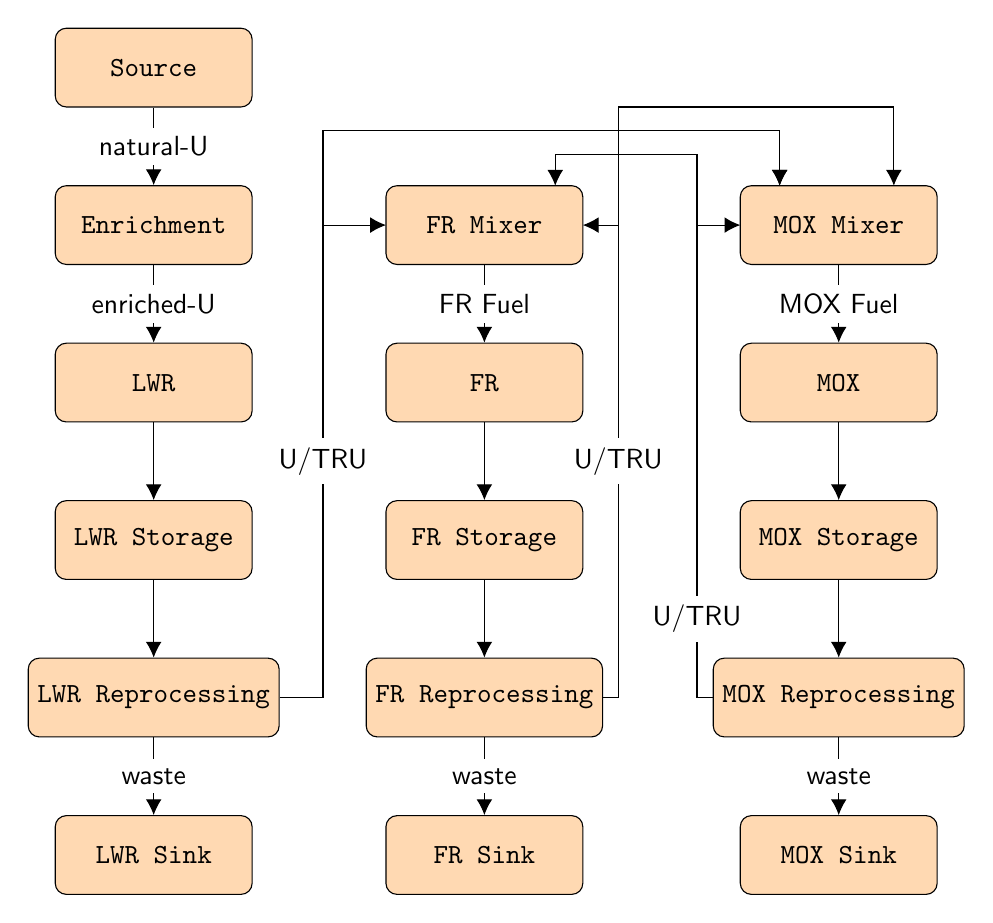
\begin{tikzpicture}[node distance=3cm,
    every node/.style={fill=white, font=\sffamily}, align=center]
  % Specification of nodes (position, etc.)
  
  \node (source)				[process] {Source};
  \node (enrichment)			[process, below of=source, yshift=1.cm] {Enrichment};
  \node (lwr)			[process, below of=enrichment, yshift=1.cm] {LWR};
  \node (lwrstorage)			[process, below of=lwr, yshift=1.cm] {LWR Storage};
  \node (lwrrepro)			[process, below of=lwrstorage, yshift=1.cm] {LWR Reprocessing};
  \node (lwrsink)			[process, below of=lwrrepro, yshift=1.cm] {LWR Sink};

  \node (frmixer)			[process, right of=enrichment, xshift=1.2cm] {FR Mixer};
  \node (fr)			[process, right of=lwr, xshift=1.2cm] {FR};
  \node (frstorage)			[process, right of=lwrstorage, xshift=1.2cm] {FR Storage};
  \node (frrepro)			[process, right of=lwrrepro, xshift=1.2cm] {FR Reprocessing};
  \node (frsink)			[process, right of=lwrsink, xshift=1.2cm] {FR Sink};

  \node (moxmixer)			[process, right of=frmixer, xshift=1.5cm] {MOX Mixer};  
  \node (mox)			[process, right of=fr, xshift=1.5cm] {MOX};
  \node (moxstorage)			[process, right of=frstorage, xshift=1.5cm] {MOX Storage};
  \node (moxrepro)			[process, right of=frrepro, xshift=1.5cm] {MOX Reprocessing};
  \node (moxsink)			[process, right of=frsink, xshift=1.5cm] {MOX Sink};

 \draw[->]					(source) -- (enrichment) node[midway] {natural-U};
 \draw[->]					(enrichment) -- (lwr) node[midway] {enriched-U};
 \draw[->]					(lwr) -- (lwrstorage);
 \draw[->]					(lwrstorage) -- (lwrrepro);
 \draw[->]					(lwrrepro) -- (lwrsink) node[midway] {waste};

 \draw[->]					(frmixer) -- (fr) node[midway] {FR Fuel};
 \draw[->]					(fr) -- (frstorage);
 \draw[->]					(frstorage) -- (frrepro);
 \draw[->]					(frrepro) -- (frsink) node[midway] {waste}; 
 
 \draw[->]					(moxmixer) -- (mox) node[midway] {MOX Fuel};
 \draw[->]					(mox) -- (moxstorage);
 \draw[->]					(moxstorage) -- (moxrepro);
 \draw[->]					(moxrepro) -- (moxsink) node[midway] {waste};

\draw[->]					(lwrrepro)++(2.15,6.)-- ++(0.,1.2)-- ++(5.8,0.)-- ++(0.,-.7);

 \draw[->]					(lwrrepro)++(1.6,0.)-- ++(0.55,0.)-- node[midway] {U/TRU} ++(0.,6.)--
  ++(0.8,0.);
 \draw[->]					(lwrrepro)++(2.15,6.)-- ++(0.,1.2)-- ++(5.8,0.)-- ++(0.,-.7);

 \draw[->]					(frrepro)++(1.5,0.)-- ++(0.2,0.)-- node[midway] {U/TRU} ++(0.,6.)--
++(-0.45,0.);
 \draw[->]					(frrepro)++(1.7,6.)-- ++(0.,1.5)--  ++(3.5,0.)-- ++(0.,-1.);

 \draw[->]					(moxrepro)++(-1.6,0.)-- ++(-0.2,0.)-- node[midway] {U/TRU} ++(0.,2.)--
++(0.,4.)-- ++(0.55,0.);  

 \draw[->]					(moxrepro)++(-1.8,6.)-- ++(0,.9)--  ++(-1.8,0.)--  ++(0.,-0.4);  

%  %\draw[->]					(refining)++(0.75,-0.5) -- ++(0,-1) -- ++(0.75,0) -| (winning);
%  \draw[->]					(refining)++(-0.75,-0.5) -- ++(0,-2)(winning) node[near start] {U/TRU + salt};
%  \draw[->]					(winning)++(0.75,0.5) -- ++(0,2) (refining) node[near start] {salt/FP/U/TRU};
%  %\draw[->]					(winning) -- ++(0,-1.25) -- ++(-2,0)  node[midway] {U} -- (fuel fab);
%  \draw[->]					(winning) -- (fuel fab) node[midway] {U/TRU};
%  \draw[->]					(reduction)++(1,-0.5) -- ++(0,-0.75) -- ++(1,0) -- ++(0,-0.75) (LiCl);
%  \draw[->]					(LiCl) -- ++(0,-1.25) -- ++(-1,0) -- ++(0,-0.75) (refining);
%  \draw[->]					(refining)++(-1,0.5) -- ++(0,0.75) -- ++(-1,0) -- ++(0,0.75) (LiCl-KCl);
%  \draw[->]					(LiCl-KCl)++(0,0.5) -- ++(0,0.75) -- ++(1,0) -- ++(0,0.75) (reduction);

  \end{tikzpicture}
\end{document}